\chapter{线虫的特征提取和急性氧化应激实验}
\section{引言}
\section{线虫的氧化急性应激实验}
	氧化应激(Oxidative Stress,OS)指生物体氧化与抗氧化作用的失衡,当生物体被内外环境中
	存在有害化合物刺激时,其体内所产生的活性氮自由基和活性氧自由基将会导致细胞或者组织发生生理和
	病理反应。过氧化氢($H_2O_2$)溶液作为一种强氧化剂经常被用于线虫的氧化应激实验中。本文
	将野生型N2秀丽隐杆线虫的L1期幼虫作为研究对象,通过本文前面介绍的软硬件平台,研究不同线性
	浓度梯度的双氧水溶液对L1期幼虫活性的影响。
\subsection{线虫的同步化}
	为了得到处于同一发育阶段的幼虫需要对线虫进行同步化处理,首先用经过高压灭菌的M9缓冲液将NGM平板上
	混合发育期的线虫冲洗到1.5ml的离心管中,离心后去掉上清液,加入碱裂解液(体积比为1:2的5N NaOH溶液和
	5\%NaClO溶液,现配),当线虫全被腐蚀时,液体将变得清澈。再经过离心处理,去掉上层碱裂解液加入M9
	缓冲液,离心洗涤1到2次。去掉上层缓冲液并用吸管将线虫卵接种到NGM平板上,至此便完成了同步化操作,等
	线虫卵孵化便得到同步化的个体。
\subsection{线性梯度稀释芯片的操作}
	图\ref{fig:sysdevice}是实验硬件部分连接示意图,芯片上所有的阀门控制和进样控制均由Arduino单片机
	通过uln2803集成芯片控制多路电磁阀实现。将含有L1期线虫的溶液离心去上清得到线虫浓缩液,
	然后用移液枪加入0.25\%的琼脂糖溶液作为线虫助悬剂。打开6号阀门,
	采用压力进样的方式将线虫溶液从4号进样口打入第三列腔室。
	打开4号阀门用压力进样的方式将水从3号进样口打入第二列腔室。
	然后打开2号阀门用压力进样的方式将30mM的过氧化氢溶液从2号进样口打入第一列腔室。
	然后关闭2号、4号和6号阀门,打开1号、3号、5号和7号阀门,
	并在一号进样口施加一个周期性的气压。通过振荡的方式使前三列腔室中的液体充分混合。
	最后通过进样口1将混合好的液体打入第四列腔室,根据芯片腔室的尺寸设计,可以计算出混合后各腔室的过氧化氢溶液的浓度从上至小依次为:
	18mM、16mM、14mM、12mM、10mM、8mM、6mM、4mM、2mM。并用CCD相机每隔10分钟采集线虫在9个腔室中的运动视频。
	\begin{figure}[h]
	  \centering
	  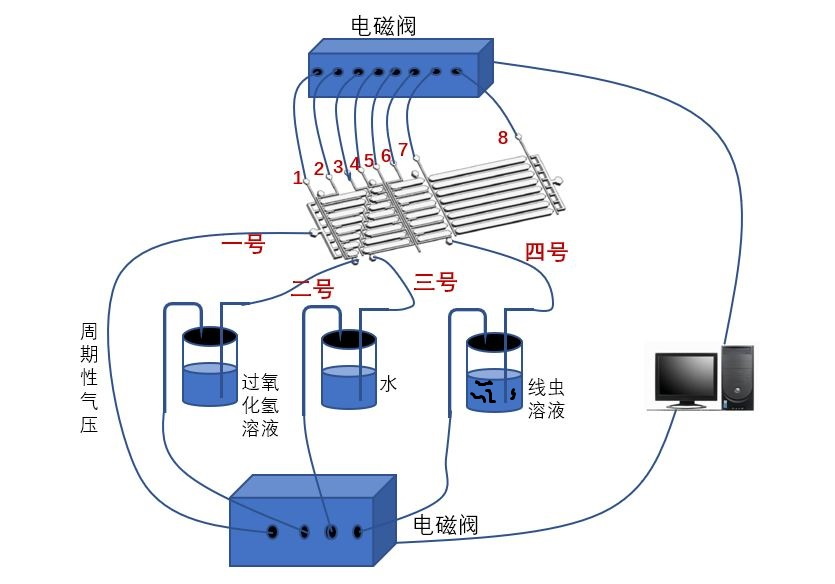
\includegraphics[width=12cm]{figure/chap5/hardware.jpg}
	  \bicaption[这里将出现在插图索引中]
		{实验系统装置示意图}
		{Change in contour curvature}
	  \label{fig:sysdevice}
	\end{figure}
\subsection{秀丽隐杆线虫急性氧化应激实验结果}
	通过本文提出的线虫轮廓分割、解析、跟踪及特征提取算法对每个腔室的各个时刻的视频进行分析并提取摆动频率特征,
	图\ref{fig:res}为了各腔室中线虫的平均摆动频率随时间的变化,可以看出随着过氧化氢溶液浓度的升高,线虫的摆动频率下降,
	且在同一浓度下,线虫的摆动频率随着时间而下降。为验证芯片实验的准确性,我们也在96孔板上手动稀释形成上述浓度后,
	通过对各个时间点线虫平均摆动频率的统计,实验结果表明96孔板实验和微流控芯片结果一致。但是相比96孔板实验,
	我们的微流控芯片平台在试剂消耗、自动分析等上面都体现了较大的优势。
	
	\begin{figure}[h]
	  \centering
	  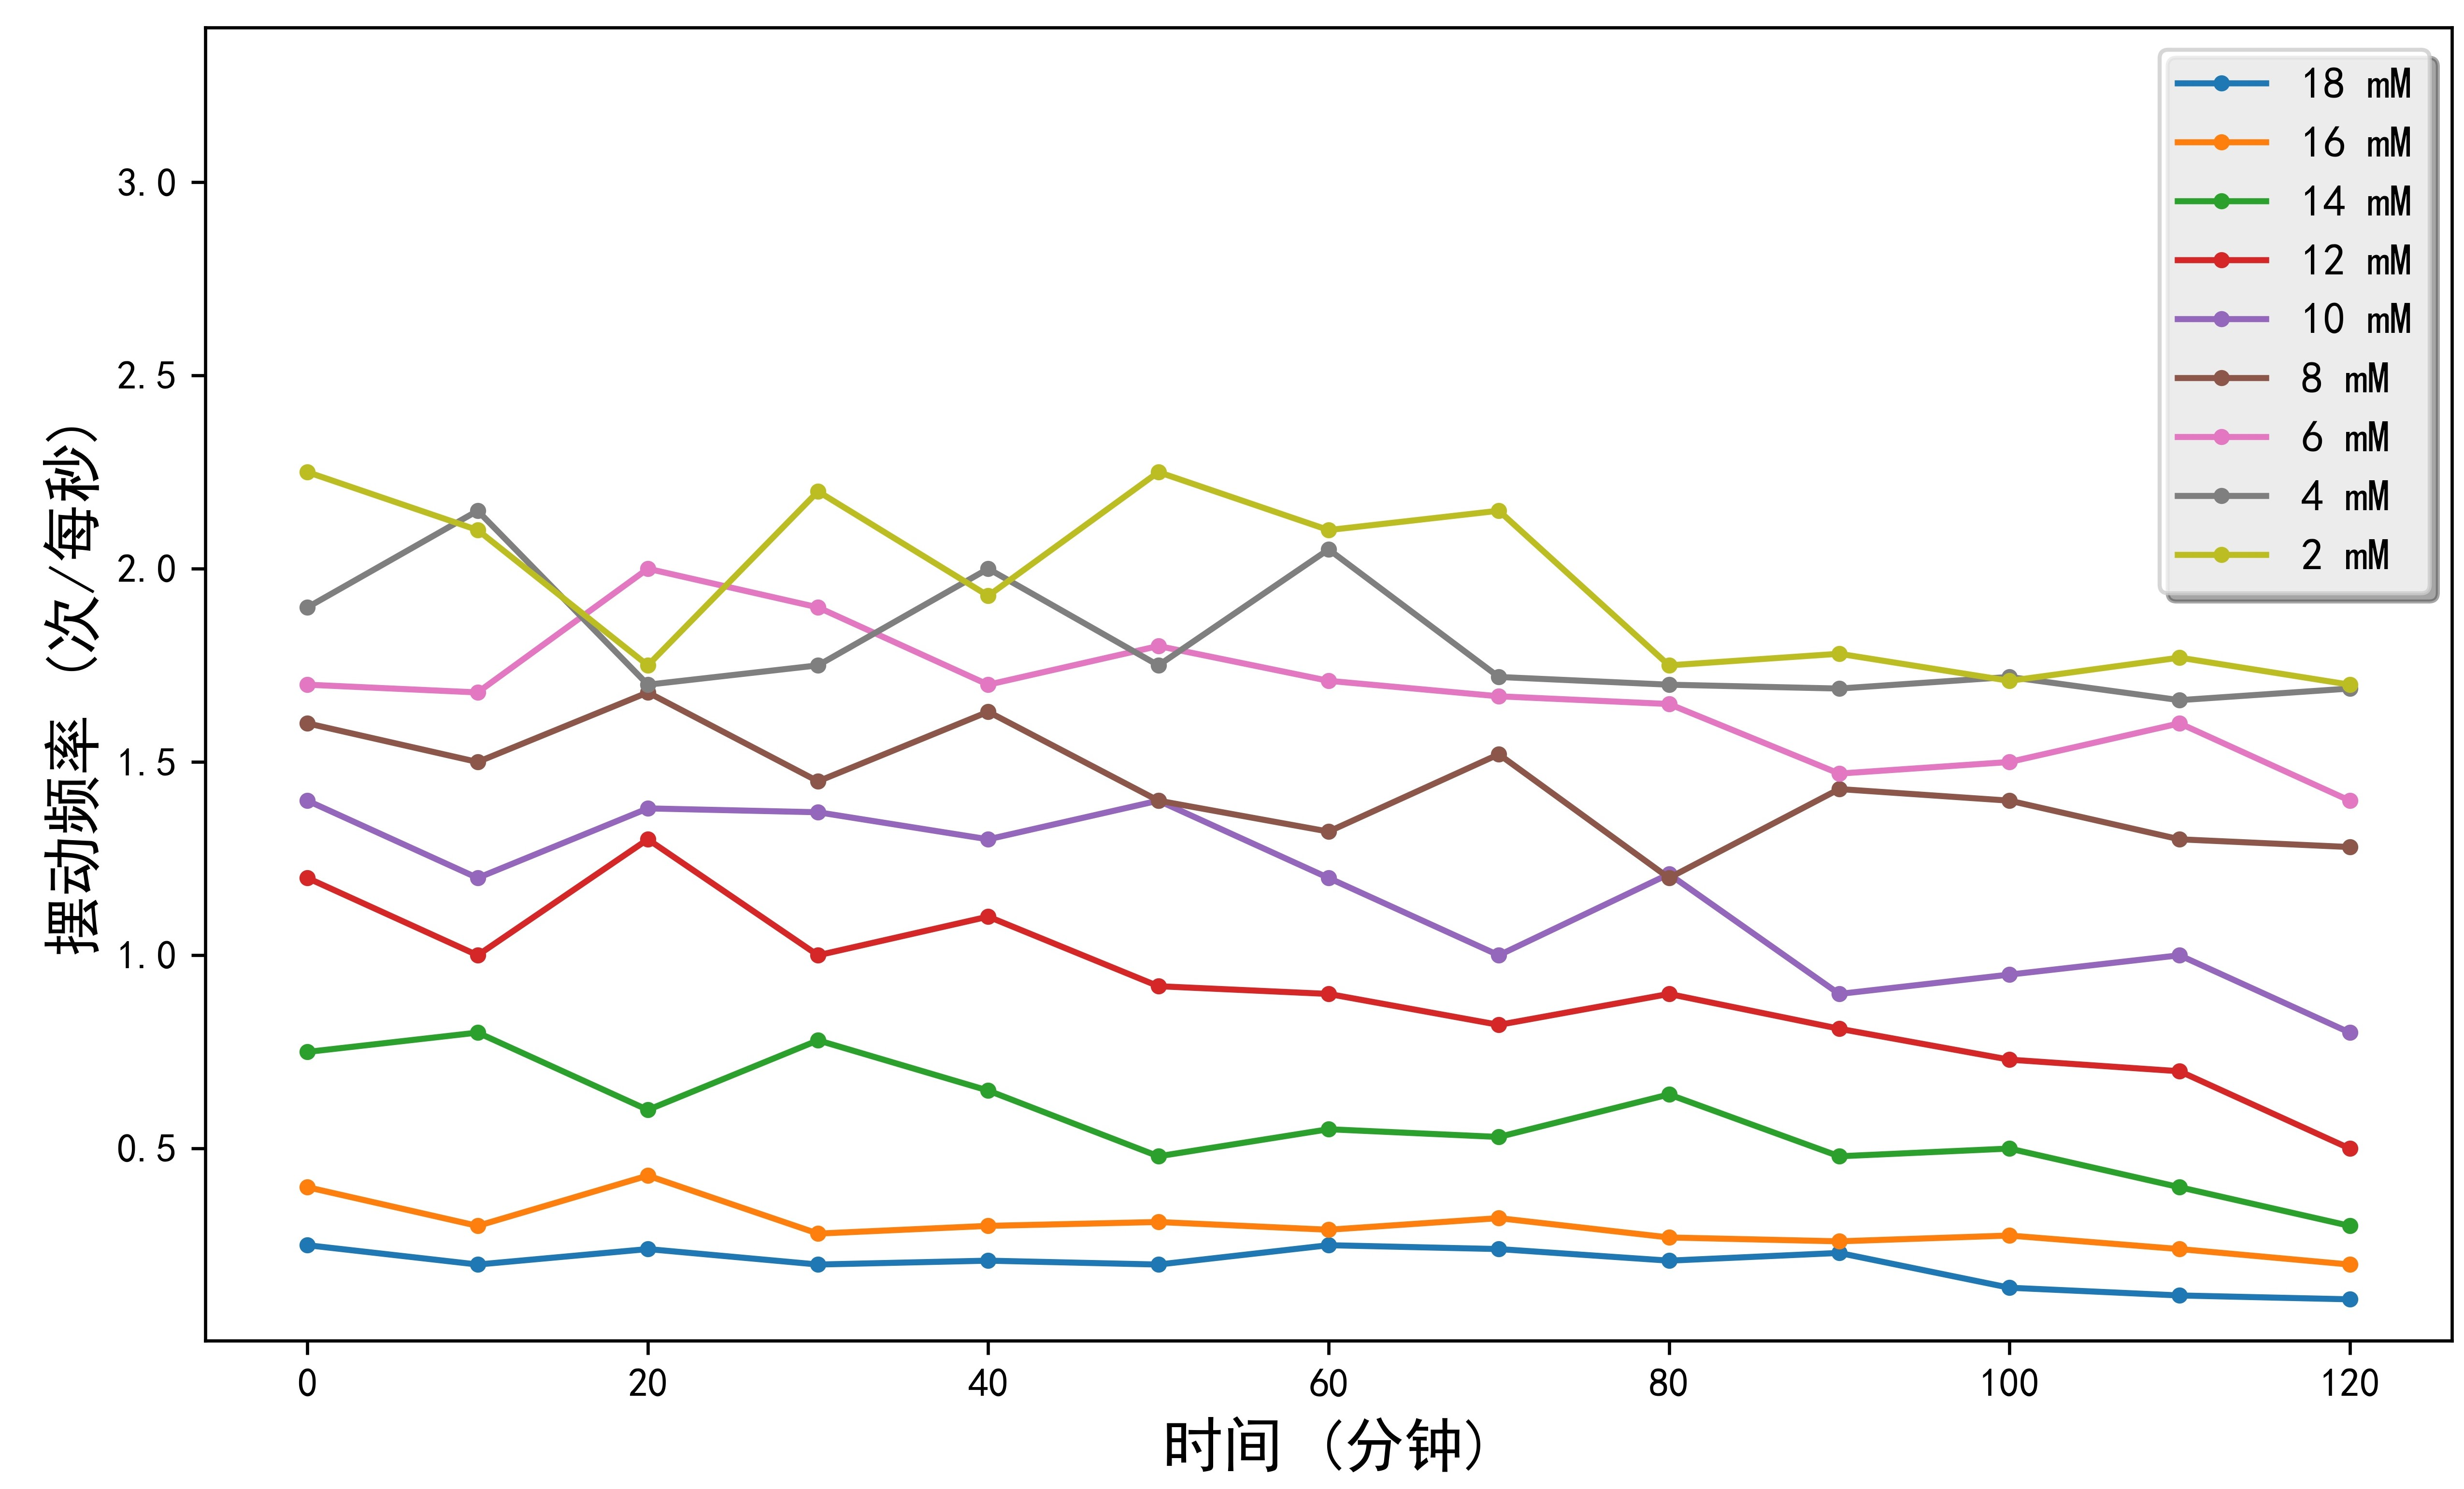
\includegraphics[width=10cm]{figure/chap5/res.jpg}
	  \bicaption[这里将出现在插图索引中]
		{各腔室中线虫平均摆动频率随时间的变化}
		{Change in contour curvature}
	  \label{fig:res}
	\end{figure}
\section{本章小结}